\documentclass[aspectratio=169]{beamer}

%------------------------------------------------
% Theme
%------------------------------------------------
\usetheme{Madrid}
\setbeamertemplate{footline}{}
\usecolortheme{dolphin}

%------------------------------------------------
% Packages
%------------------------------------------------
\usepackage{amsmath,amssymb}
\usepackage{tikz}
\usetikzlibrary{positioning,shapes.geometric,arrows.meta}
\usepackage{booktabs}
\usepackage{array}
\usetikzlibrary{patterns}

%------------------------------------------------
% Title
%------------------------------------------------
\title{Mathematics for Computing}

\author{Adarsh P Kurian}

\institute{
Department of Computer Science and Engineering\\
Cochin University of Science and Technology(CUSAT)\\[0.2cm]
M.Tech in Computer Science and Engineering\\
(Artificial Intelligence and Software Engineering)\\
Semester I
}

\date{6 August, 2026}

\begin{document}

%%%%%%%%%%%%%%%%%%%%%%%%%%%%%%%%%%%%%%%%%%%%%%%%%%
\begin{frame}
\titlepage
\end{frame}

%%%%%%%%%%%%%%%%%%%%%%%%%%%%%%%%%%%%%%%%%%%%%%%%%%
\begin{frame}{What is a Set?}

\textbf{Definition}

A set is a well-defined collection of distinct objects called
\textbf{elements}.

\vspace{0.3cm}

Mathematically,

\[
A=\{a_1,a_2,a_3,\ldots,a_n\}
\]

where every element is unique.

\vspace{0.4cm}

\textbf{Why are Sets Important in AI?}

\begin{itemize}
\item Represent datasets
\item Store detected objects
\item Represent feature sets
\item Query databases
\item Build recommendation systems
\item Define search spaces
\item Knowledge representation
\end{itemize}

\end{frame}

%%%%%%%%%%%%%%%%%%%%%%%%%%%%%%%%%%%%%%%%%%%%%%%%%%
%%%%%%%%%%%%%%%%%%%%%%%%%%%%%%%%%%%%%%%%%%%%%%%%%%
\begin{frame}{10 Examples in Set-Builder and Roster Form}

\scriptsize

\begin{table}
\centering

\begin{tabular}{c p{6.3cm} p{5.0cm}}

\toprule
\textbf{No.} &
\textbf{Set-Builder Form} &
\textbf{Roster / Extended Form}
\\





1 &
$
A = \{ (-1)^{n+1} \cdot n^2 \mid n \in \mathbb{N} \}
$
&
$
\{1, -4, 9, -16, 25, -36, \ldots\}
$
\\[0.18cm]

2 &
$
B = \left\{ \frac{n}{n+1} \;\middle|\; n \in \mathbb{N}, \, 1 \le n \le 5 \right\}
$
&
$
\left\{ \frac{1}{2}, \frac{2}{3}, \frac{3}{4}, \frac{4}{5}, \frac{5}{6} \right\}
$
\\[0.18cm]

3 &
$
C = \{ x\in \mathbb{N} \mid 3 \mid x \land 5 \nmid x \}
$
&
$
\{3, 6, 9, 12, 18, 21, 24, \ldots\}
$
\\[0.18cm]

4 &
$
D = \{ x \in \mathbb{Z} \mid 1 \le |x| \le 3 \}
$
&
$
\{-3, -2, -1, 1, 2, 3\}
$
\\[0.18cm]

5 &
$
E = \{ w \in \{a, b\}^* \mid |w| \pmod 2 = 0 \}
$
&
$
\{\varepsilon, aa, ab, ba, bb, aaaa, \ldots\}
$
\\[0.18cm]



6 &
$
F = \{ x \in \mathbb{Z}_{12}^+ \mid \gcd(x, 12) = 1 \}
$
&
$
\{1, 5, 7, 11\} \quad (\text{Units of } \mathbb{Z}_{12})
$
\\[0.18cm]

7 &
$
G = \{ (x, y) \in \mathbb{Z} \times \mathbb{Z} \mid x^2 + y^2 = 25 \}
$
&
$
\{(0, \pm 5), (\pm 5, 0), (\pm 3, \pm 4), (\pm 4, \pm 3)\}
$
\\[0.18cm]

8 &
$
H = \left\{ \frac{1+(-1)^n}{2 \cdot n} \;\middle|\; n \in \mathbb{N} \right\}
$
&
$
\left\{ 0, \frac{1}{2}, 0, \frac{1}{4}, 0, \frac{1}{6}, \ldots \right\}
$
\\[0.18cm]

9 &
$
I = \{ a^n b^n c^n \mid n \in \mathbb{Z}_{\ge 0} \}
$
&
$
\{\varepsilon, abc, aabbcc, aaabbbccc, \ldots\}
$
\\[0.18cm]

10 &
$
J = \{ w \in \{a, b\}^* \mid w = w^R \}
$
&
$
\{\varepsilon, a, b, aa, bb, aba, bab, \ldots\}
$
\\

\bottomrule

\end{tabular}

\end{table}

\end{frame}
%%%%%%%%%%%%%%%%%%%%%%%%%%%%%%%%%%%%%%%%%%%%%%%%%%

%%%%%%%%%%%%%%%%%%%%%%%%%%%%%%%%%%%%%%%%%%%%%%%%%%
%%%%%%%%%%%%%%%%%%%%%%%%%%%%%%%%%%%%%%%%%%%%%%%%%%
\begin{frame}{Cardinality of a Set}

\textbf{Definition}

The cardinality of a set is the number of distinct elements in the set.

\vspace{0.3cm}

\textbf{Mathematical Expression}

\[
|A|=n
\]

where \(n\) is the number of elements in \(A\).

\vspace{0.4cm}

\textbf{AI Example}

Suppose a YOLO object detection model detects the following objects in an image:

\[
D=
\{
Car_1,\;
Car_2,\;
Person_1,\;
TrafficLight_1,\;
Bus_1
\}
\]

Therefore,

\[
|D|=5
\]

\textbf{Interpretation:} The model detected \textbf{5 unique objects}.

\end{frame}
%%%%%%%%%%%%%%%%%%%%%%%%%%%%%%%%%%%%%%%%%%%%%%%%%%


%%%%%%%%%%%%%%%%%%%%%%%%%%%%%%%%%%%%%%%%%%%%%%%%%%
\begin{frame}{Finite Set}

\textbf{Definition}

A finite set is a set containing a limited (countable) number of elements.

\vspace{0.3cm}

\textbf{Mathematical Expression}

\[
A=\{x\in\mathbb{N}\mid x\le5\}
=\{1,2,3,4,5\}
\]

\[
|A|=5
\]

\vspace{0.4cm}

\textbf{AI Practical Example}

In a sentiment analysis model, each review is classified into one of three sentiment classes.

\[
Sentiment=
\{
Positive,\;
Neutral,\;
Negative
\}
\]

\[
|Sentiment|=3
\]

Since the number of sentiment classes is limited, \textbf{Sentiment} is a finite set.

\end{frame}
%%%%%%%%%%%%%%%%%%%%%%%%%%%%%%%%%%%%%%%%%%%%%%%%%%
%%%%%%%%%%%%%%%%%%%%%%%%%%%%%%%%%%%%%%%%%%%%%%%%%%
%%%%%%%%%%%%%%%%%%%%%%%%%%%%%%%%%%%%%%%%%%%%%%%%%%
\begin{frame}{Infinite Set}

\textbf{Definition}

An infinite set contains an unlimited number of elements.

\vspace{0.3cm}

\textbf{Mathematical Expression}

\[
A=\{x\in\mathbb N\}
=\{1,2,3,\ldots\}
\]

\vspace{0.3cm}

\textbf{AI Practical Example}

An autonomous vehicle continuously generates LiDAR scans.

\[
L=\{P_1,P_2,P_3,\ldots\}
\]

where \(P_i\) denotes the \(i^{th}\) LiDAR scan.

Since new scans are continuously generated,

\[
L \text{ is treated as an infinite set.}
\]

\end{frame}
%%%%%%%%%%%%%%%%%%%%%%%%%%%%%%%%%%%%%%%%%%%%%%%%%%

%%%%%%%%%%%%%%%%%%%%%%%%%%%%%%%%%%%%%%%%%%%%%%%%%%
\begin{frame}{Null (Empty) Set}

\textbf{Definition}

A null (empty) set contains no elements.

\vspace{0.4cm}

\textbf{Mathematical Expression}

\[
A=\{x\in\mathbb N\mid x<0\}
=\emptyset
\]

\vspace{0.4cm}

\textbf{Practical AI Example}

An object detection model analyzes an empty parking lot.

Detected vehicles

\[
DetectedCars=\emptyset
\]

Cardinality

\[
|DetectedCars|=0
\]

The model correctly detects no vehicles.
\vspace{0.3cm}


\end{frame}

%%%%%%%%%%%%%%%%%%%%%%%%%%%%%%%%%%%%%%%%%%%%%%%%%%
\begin{frame}{Equal Sets}

\textbf{Definition}

Two sets are equal if they contain exactly the same elements.

\[
A=B
\iff
\forall x,\; (x\in A \Leftrightarrow x\in B)
\]

\vspace{0.3cm}

\textbf{AI Example}

\[
GT=\{Car,\;Person,\;TrafficLight\}
\]

\[
P=\{TrafficLight,\;Person,\;Car\}
\]

\[
GT=P
\]

\centering
\textbf{Both sets contain identical labels.}

\end{frame}
%%%%%%%%%%%%%%%%%%%%%%%%%%%%%%%%%%%%%%%%%%%%%%%%%%
%%%%%%%%%%%%%%%%%%%%%%%%%%%%%%%%%%%%%%%%%%%%%%%%%%
\begin{frame}{Equivalent Sets}

\textbf{Definition}

Two sets are equivalent if they contain the same number of elements.

\[
|A|=|B|
\]

\vspace{0.4cm}

\textbf{Practical AI Example}

Training Dataset

\[
Cats=
\{
I_1,I_2,\ldots,I_{5000}
\}
\]

Validation Dataset

\[
Dogs=
\{
J_1,J_2,\ldots,J_{5000}
\}
\]

Although images are different,

\[
|Cats|=|Dogs|=5000
\]

Hence the datasets are equivalent.

\vspace{0.3cm}

Balanced datasets improve machine learning performance.

\end{frame}

%%%%%%%%%%%%%%%%%%%%%%%%%%%%%%%%%%%%%%%%%%%%%%%%%%
\begin{frame}{Countable Set}

\textbf{Definition}

A set is countable if its elements can be placed in one-to-one correspondence with the natural numbers.

\vspace{0.3cm}

\[
A=\{a_1,a_2,a_3,\cdots\}
\]

\vspace{0.4cm}

\textbf{Practical AI Example}

Every image in a dataset receives a unique ID.

\[
Images=
\{
Img_1,
Img_2,
Img_3,
\cdots
\}
\]

Examples

\begin{itemize}
\item CIFAR-10
\item COCO Dataset
\end{itemize}

Each image can be indexed uniquely.

Hence the dataset is countable.

\end{frame}

%%%%%%%%%%%%%%%%%%%%%%%%%%%%%%%%%%%%%%%%%%%%%%%%%%
\begin{frame}{Power Set}

\textbf{Definition}

The power set of a set \(A\) is the set of all subsets of \(A\).

\[
\mathcal{P}(A)=\{S\mid S\subseteq A\}
\]

If \(|A|=n\),

\[
|\mathcal{P}(A)|=2^n
\]

\vspace{0.3cm}

\textbf{AI Practical Example}

Features used for training:

\[
F=\{Age,\;Income,\;CreditScore\}
\]

Possible feature subsets include

\[
\emptyset,\;
\{Age\},\;
\{Age,Income\},\;
\{Income,CreditScore\},\;
\ldots,\;
\{Age,Income,CreditScore\}
\]

Since there are 3 features,

\[
|\mathcal{P}(F)|=2^3=8
\]

These subsets are evaluated during exhaustive feature selection.

\end{frame}
%%%%%%%%%%%%%%%%%%%%%%%%%%%%%%%%%%%%%%%%%%%%%%%%%%

%%%%%%%%%%%%%%%%%%%%%%%%%%%%%%%%%%%%%%%%%%%%%%%%%%
\begin{frame}{Subset}

\textbf{Definition}

A set \(A\) is a subset of \(B\) if every element of \(A\) belongs to \(B\).

\vspace{0.2cm}

\[
A\subseteq B
\]

\vspace{0.2cm}

\textbf{AI Practical Example}

All transactions:

\[
T=\{T_1,T_2,T_3,T_4,T_5\}
\]

Fraudulent transactions:

\[
F=\{T_2,T_5\}
\]

Therefore,

\[
F\subseteq T
\]

\textbf{Interpretation:} Every fraudulent transaction belongs to the set of all transactions.

\end{frame}
%%%%%%%%%%%%%%%%%%%%%%%%%%%%%%%%%%%%%%%%%%%%%%%%%%
%%%%%%%%%%%%%%%%%%%%%%%%%%%%%%%%%%%%%%%%%%%%%%%%%%
\begin{frame}{Universal Set}

\textbf{Definition}

The universal set contains all elements under consideration.

\vspace{0.3cm}

\[
U=\{x \mid x \text{ belongs to the sample space}\}
\]

\vspace{0.3cm}

\textbf{Practical AI Example: Image Classification Dataset}

Suppose a computer vision dataset contains images from five classes.

\[
U=
\{
Cat,
Dog,
Car,
Person,
TrafficLight
\}
\]

A CNN classifier can predict only one of these classes.

\vspace{0.3cm}

Example subsets:

\[
Animals=\{Cat,Dog\}
\]

\[
RoadObjects=\{Car,TrafficLight\}
\]

Both are subsets of the universal set.

\vspace{0.4cm}

Applications

\begin{itemize}
\item Image Classification
\item Object Detection
\item Dataset Organization
\item Label Management
\end{itemize}

\end{frame}

%%%%%%%%%%%%%%%%%%%%%%%%%%%%%%%%%%%%%%%%%%%%%%%%%%
\begin{frame}{Singleton Set}

\textbf{Definition}

A singleton set contains exactly one element.

\[
|A|=1
\]



\vspace{0.2cm}

\textbf{Practical AI Example}

A face recognition system identifies only one person in an image.

Prediction

\[
Recognized=
\{Tony\}
\]

Therefore



is a singleton set.

\end{frame}

%%%%%%%%%%%%%%%%%%%%%%%%%%%%%%%%%%%%%%%%%%%%%%%%%%
\begin{frame}{Union of Two Sets}

\textbf{Definition}

The union contains every element belonging to either set.

\[
A\cup B
=
\{x \mid x\in A \text{ or } x\in B\}
\]

\vspace{0.4cm}

\textbf{Practical AI Example}

Two object detection models analyze the same image.

YOLO detects

\[
Y=
\{
Car,
Person,
Bus
\}
\]

Mask R-CNN detects

\[
M=
\{
Person,
Bike,
TrafficLight
\}
\]

Combined detections

\[
Y\cup M
=
\{
Car,
Person,
Bus,
Bike,
TrafficLight
\}
\]

\vspace{0.3cm}

This represents every object detected by at least one model.

\vspace{0.2cm}

\begin{center}
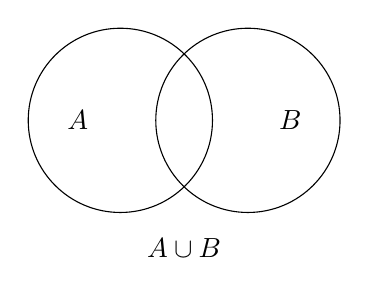
\begin{tikzpicture}[scale=0.9]

\draw (0,0) circle (1.3);
\draw (1.8,0) circle (1.3);

\node at (-0.6,0) {$A$};
\node at (2.4,0) {$B$};

\node at (0.9,-1.8) {$A\cup B$};

\end{tikzpicture}
\end{center}

\end{frame}

%%%%%%%%%%%%%%%%%%%%%%%%%%%%%%%%%%%%%%%%%%%%%%%%%%
\begin{frame}{Intersection of Two Sets}

\textbf{Definition}

The intersection of two sets contains the elements common to both sets.

\[
A\cap B=\{x\mid x\in A \text{ and } x\in B\}
\]

\vspace{0.3cm}

\textbf{AI Practical Example}

Movies liked by User A:

\[
A=\{M_1,M_2,M_3,M_5\}
\]

Movies liked by User B:

\[
B=\{M_2,M_3,M_4\}
\]

\[
A\cap B=\{M_2,M_3\}
\]

\textbf{Interpretation:} These common movies can improve collaborative recommendations.

\end{frame}
%%%%%%%%%%%%%%%%%%%%%%%%%%%%%%%%%%%%%%%%%%%%%%%%%%

%%%%%%%%%%%%%%%%%%%%%%%%%%%%%%%%%%%%%%%%%%%%%%%%%%
\begin{frame}{Set Difference}

\textbf{Definition}

The difference of two sets contains elements in the first set but not in the second.

\[
A-B=\{x\mid x\in A,\;x\notin B\}
\]

\textbf{AI Practical Example}

\[
M=\{M_1,M_2,M_3,M_4,M_5\}
\]

\[
W=\{M_2,M_4\}
\]

\[
M-W=\{M_1,M_3,M_5\}
\]

\textbf{Interpretation:} Recommend movies not yet watched.



\end{frame}
%%%%%%%%%%%%%%%%%%%%%%%%%%%%%%%%%%%%%%%%%%%%%%%%%%
%%%%%%%%%%%%%%%%%%%%%%%%%%%%%%%%%%%%%%%%%%%%%%%%%%
\begin{frame}{Symmetric Difference}

\textbf{Definition}

The symmetric difference contains elements that belong to exactly one of the two sets.

\[
A\triangle B=(A-B)\cup(B-A)
\]

\vspace{0.3cm}

\textbf{AI Practical Example}

Features selected by LASSO:

\[
L=\{Age,\;Income,\;CreditScore\}
\]

Features selected by Decision Tree:

\[
D=\{Income,\;Education,\;Experience\}
\]

\[
L\triangle D=
\{Age,\;CreditScore,\;Education,\;Experience\}
\]

\textbf{Interpretation:} These features are selected by only one of the two algorithms.

\end{frame}
%%%%%%%%%%%%%%%%%%%%%%%%%%%%%%%%%%%%%%%%%%%%%%%%%%
%%%%%%%%%%%%%%%%%%%%%%%%%%%%%%%%%%%%%%%%%%%%%%%%%%
\begin{frame}{Complement}

\textbf{Definition}

The complement of a set contains every element of the
universal set except those in the given set.

\[
A^c
=
U-A
\]

\vspace{0.4cm}

\textbf{Practical AI Example}

Universal Set

\[
U=
\{
All\ Emails
\}
\]

Spam Emails

\[
S=
\{
Spam
\}
\]

Complement

\[
S^c
=
NonSpam
\]

Spam classifiers such as Naive Bayes, SVM and
Transformer-based models classify emails into

\[
Spam
\quad\text{or}\quad
NonSpam
\]

where

\[
NonSpam=S^c
\]







\end{frame}

%%%%%%%%%%%%%%%%%%%%%%%%%%%%%%%%%%%%%%%%%%%%%%%%%%
\begin{frame}{Cartesian Product}

\textbf{Definition}

The Cartesian product is the set of all ordered pairs.

\[
A\times B=\{(a,b)\mid a\in A,\;b\in B\}
\]

\vspace{0.3cm}

\textbf{AI Practical Example}

Images:

\[
I=\{Image_1,Image_2\}
\]

Languages:

\[
L=\{English,Spanish\}
\]

\[
I\times L=
\{
(Image_1,English),
(Image_1,Spanish),
(Image_2,English),
(Image_2,Spanish)
\}
\]

\textbf{Interpretation:} Each pair represents generating a caption for an image in a specific language.

\end{frame}
%%%%%%%%%%%%%%%%%%%%%%%%%%%%%%%%%%%%%%%%%%%%%%%%%%
%%%%%%%%%%%%%%%%%%%%%%%%%%%%%%%%%%%%%%%%%%%%%%%%%%
\begin{frame}{General Form of Inclusion--Exclusion Principle}

\textbf{Definition}

The Inclusion--Exclusion Principle computes the total number of
distinct elements present in the union of several overlapping sets.

\vspace{0.3cm}

For two sets,

\[
|A\cup B|
=
|A|+|B|-|A\cap B|
\]

\vspace{0.3cm}

For three sets,

\[
|A\cup B\cup C|
=
|A|+|B|+|C|
-|A\cap B|
-|A\cap C|
-|B\cap C|
+|A\cap B\cap C|
\]

\vspace{0.3cm}

General Formula

\[
\left|
\bigcup_{i=1}^{n}A_i
\right|
=
\sum |A_i|
-
\sum |A_i\cap A_j|
+
\sum |A_i\cap A_j\cap A_k|
-\cdots
+(-1)^{n+1}
\left|
\bigcap_{i=1}^{n}A_i
\right|
\]

\vspace{0.3cm}


\end{frame}

%%%%%%%%%%%%%%%%%%%%%%%%%%%%%%%%%%%%%%%%%%%%%%%%%%
%%%%%%%%%%%%%%%%%%%%%%%%%%%%%%%%%%%%%%%%%%%%%%%%%%
\begin{frame}{Relation}

\textbf{Definition}

A relation \(R\) from \(A\) to \(B\) is a set of ordered pairs
where elements of \(A\) are related to elements of \(B\).

\[
R\subseteq A\times B
\]

\vspace{0.2cm}

\textbf{Data Science Example: Customer--Product Relation}
Customers:
\[
C=\{C_1,C_2,C_3\}
\]
Products:
\[
P=\{P_1,P_2,P_3\}
\]
Suppose customers purchased products:
\[
R=\{(C_1,P_1),(C_1,P_3),(C_2,P_2),(C_3,P_1)\}
\]
\[
R\subseteq C\times P
\]
\textbf{Interpretation:} Each pair represents a customer--product
purchase and can be used for recommendation systems.

\end{frame}
%%%%%%%%%%%%%%%%%%%%%%%%%%%%%%%%%%%%%%%%%%%%%%%%%%
%%%%%%%%%%%%%%%%%%%%%%%%%%%%%%%%%%%%%%%%%%%%%%%%%%
\begin{frame}{Equivalence Relation}

\textbf{Definition}

A relation \(R\) is an \textbf{equivalence relation} if it is

\[
\boxed{\text{Reflexive, Symmetric, and Transitive}}
\]

\vspace{0.2cm}
\textbf{Data Science Example: Customer Records}
Let
\[
D=\{d_1,d_2,d_3,d_4\}
\]
Define
\[
d_iRd_j
\iff
\text{CustomerID}(d_i)=\text{CustomerID}(d_j)
\]
Suppose
\[
ID(d_1)=ID(d_3)=101
\]
\[
ID(d_2)=ID(d_4)=102
\]
Then
\[
[d_1]=\{d_1,d_3\},
\qquad
[d_2]=\{d_2,d_4\}
\]
\textbf{Interpretation:} Records with the same Customer ID
belong to the same equivalence class.

\end{frame}
%%%%%%%%%%%%%%%%%%%%%%%%%%%%%%%%%%%%%%%%%%%%%%%%%%
%%%%%%%%%%%%%%%%%%%%%%%%%%%%%%%%%%%%%%%%%%%%%%%%%%
\begin{frame}{Partially Ordered Set (Poset)}

\textbf{Definition}

A relation \(R\) on a set \(A\) is a \textbf{partial order} if it is

\begin{itemize}
\item Reflexive
\item Antisymmetric
\item Transitive
\end{itemize}

Then \((A,R)\) is called a \textbf{Partially Ordered Set (Poset)}.

\vspace{0.2cm}

\textbf{Example}

Let

\[
A=\{1,2,3,4,5\},\qquad
aRb \iff a\le b
\]

Examples:

\[
1\le2,\;
2\le4,\;
3\le5,\;
1\le5
\]

Since every pair of elements is comparable under \(\le\), this relation is a partial order (in fact, a total order).
Hence, \((A,R)\) is a \textbf{Poset}.

\end{frame}
%%%%%%%%%%%%%%%%%%%%%%%%%%%%%%%%%%%%%%%%%%%%%%%%%%
%%%%%%%%%%%%%%%%%%%%%%%%%%%%%%%%%%%%%%%%%%%%%%%%%%
\begin{frame}{Hasse Diagram of a Poset}

Let

\[
A=\{1,2,3,4,5\},\qquad aRb\iff a\le b
\]

\begin{center}

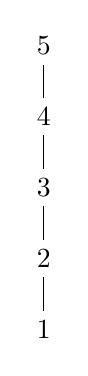
\begin{tikzpicture}[scale=0.9]

\node (1) at (0,0){1};
\node (2) at (0,1){2};
\node (3) at (0,2){3};
\node (4) at (0,3){4};
\node (5) at (0,4){5};

\draw (1)--(2);
\draw (2)--(3);
\draw (3)--(4);
\draw (4)--(5);

\end{tikzpicture}

\end{center}

\[
1\prec2\prec3\prec4\prec5
\]

\centering
\textbf{This Hasse diagram forms a chain (total order).}

\end{frame}
%%%%%%%%%%%%%%%%%%%%%%%%%%%%%%%%%%%%%%%%%%%%%%%%%%
%%%%%%%%%%%%%%%%%%%%%%%%%%%%%%%%%%%%%%%%%%%%%%%%%%
\begin{frame}{Power Set Ordered by Subset Relation}

Consider

\[
A=\{1,2,3\}
\]

Its power set is

\[
P(A)=
\{
\emptyset,
\{1\},
\{2\},
\{3\},
\{1,2\},
\{1,3\},
\{2,3\},
\{1,2,3\}
\}
\]

Define the relation

\[
S_iRS_j
\iff
S_i\subseteq S_j
\]


\[
(P(A),\subseteq)
\]

forms a \textbf{Partially Ordered Set (Poset)}.

\vspace{0.3cm}


\end{frame}

%%%%%%%%%%%%%%%%%%%%%%%%%%%%%%%%%%%%%%%%%%%%%%%%%%
%%%%%%%%%%%%%%%%%%%%%%%%%%%%%%%%%%%%%%%%%%%%%%%%%%
\begin{frame}{Hasse Diagram of the Power Set}

\[
A=\{1,2,3\},\qquad R=\subseteq
\]

\begin{center}

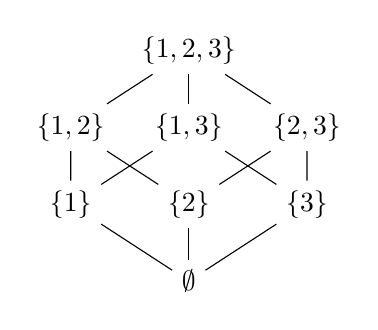
\begin{tikzpicture}[scale=0.75]

\node (0)   at (0,0) {$\emptyset$};

\node (1)   at (-2,1.3) {$\{1\}$};
\node (2)   at (0,1.3) {$\{2\}$};
\node (3)   at (2,1.3) {$\{3\}$};

\node (12)  at (-2,2.6) {$\{1,2\}$};
\node (13)  at (0,2.6) {$\{1,3\}$};
\node (23)  at (2,2.6) {$\{2,3\}$};

\node (123) at (0,3.9) {$\{1,2,3\}$};

\draw (0)--(1);
\draw (0)--(2);
\draw (0)--(3);

\draw (1)--(12);
\draw (1)--(13);

\draw (2)--(12);
\draw (2)--(23);

\draw (3)--(13);
\draw (3)--(23);

\draw (12)--(123);
\draw (13)--(123);
\draw (23)--(123);

\end{tikzpicture}

\end{center}

\centering
\small Hasse diagram of the power set ordered by the subset relation.

\end{frame}
%%%%%%%%%%%%%%%%%%%%%%%%%%%%%%%%%%%%%%%%%%%%%%%%%%
\begin{frame}{Chain}

\textbf{Definition}

A subset \(C\) of a Poset is called a \textbf{chain} if every
pair of elements in \(C\) is comparable.

\[
\forall a,b\in C,\qquad
a\le b\;\text{or}\;b\le a
\]

\vspace{0.2cm}

\textbf{Example}

Let

\[
A=\{1,2,3,4,5\},\qquad aRb\iff a\le b
\]

Consider
\[
C=\{1,3,5\}
\]

Since

\[
1<3<5
\]
every pair of elements is comparable.
\[
\boxed{C\text{ is a Chain}}
\]

\end{frame}
%%%%%%%%%%%%%%%%%%%%%%%%%%%%%%%%%%%%%%%%%%%%%%%%%%
%%%%%%%%%%%%%%%%%%%%%%%%%%%%%%%%%%%%%%%%%%%%%%%%%%
\begin{frame}{Antichain}

\textbf{Definition}

A subset \(S\) of a Poset is called an \textbf{antichain} if no
two distinct elements of \(S\) are comparable.

\[
a\ne b\Rightarrow
a\nleq b\;\text{and}\;b\nleq a
\]

\vspace{0.2cm}

\textbf{Example}

Let
\[
A=\mathcal{P}(\{1,2,3\})
\]
ordered by the subset relation \(\subseteq\).
Consider
\[
S=\{\{1\},\{2\},\{3\}\}
\]
Since
\[
\{1\}\nsubseteq\{2\},\qquad
\{2\}\nsubseteq\{3\},\qquad
\{1\}\nsubseteq\{3\}
\]

no two elements are comparable.

\[
\boxed{S\text{ is an Antichain}}
\]

\end{frame}

%%%%%%%%%%%%%%%%%%%%%%%%%%%%%%%%%%%%%%%%%%%%%%%%%%
\begin{frame}{}

\textbf{Thank You!}\centering

\end{frame}

%%%%%%%%%%%%%%%%%%%%%%%%%%%%%%%%%%%%%%%%%%%%%%%%%%

\end{document}
